\section{Introduction}
Everyone trusts the timestamps recorded on the
blockchain are accurate. But why?
In the original Bitcoin paper~\cite{bitcoin}, Nakamoto refers to the
blockchain as a distributed timestamping server.
Applications rely on the precision of these recorded timestamps.
For example, DeFi applications rely~\cite{0x-timestamp} on new transactions not only
being included soon (a well-understood property known as \emph{liveness}),
but also that the timestamps they are recorded with are relatively fresh.

However, timestamps in adversarially produced blocks may be fabricated.
And yet, empirical evidence suggests reported timestamps roughly correspond
to real world time.

In this paper, we put forth the notion of \emph{timeliness}, formalizing the folklore
understanding that timestamps recorded on-chain cannot deviate arbitrarily
from real world time. In particular we define a timeliness parameter $v$ which bounds
this potential deviation. Under honest majority, we prove this virtue materializes in all three popular flavors of
permissionless blockchains, namely proof-of-work,
longest chain proof-of-stake, and quorum-based proof-of-stake, and calculate the
timeliness parameter.

Blockchain systems executed in networks with delay, even when assuming a global clock and
a synchronous network, allow honest parties to reach consensus, but not at exactly
the same time. We observe that any timely blockchain can be modified to achieve
consensus at the same exact global time, a property we call \emph{supersafety},
albeit with the introduction of a small confirmation delay. We posit that the introduction of this
property in this abstract fashion greatly simplifies the proofs of security of protocols built on top.

\noindent
\textbf{Our contributions.}

\begin{enumerate}
  \item We define the notion of \emph{timeliness} of a blockchain system.
  \item We prove that three exemplary cases of blockchain protocols (Bitcoin, Streamlet, and Ouroboros)
        are timely and calculate their timeliness parameter.
  \item We prove that timeliness cannot be achieved in partial synchrony before GST.
  \item We present a black-box reduction from \emph{timeliness} to \emph{supersafety} and back,
        remaining mindful of late-joining clients.
\end{enumerate}

\begin{figure}
  \centering
  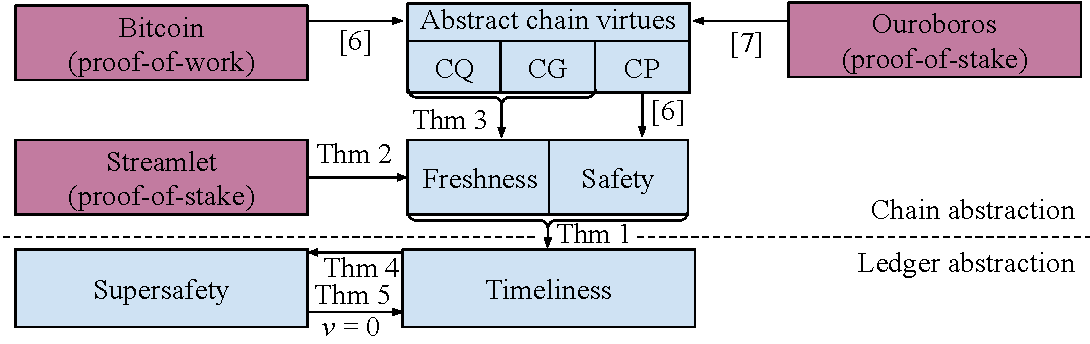
\includegraphics[width=1.0\columnwidth,keepaspectratio]{figures/timeliness-overview.pdf}
  \caption{Overview of the paper. Bitcoin and Ouroboros attain the abstract chain virtues
  of Common Prefix, Chain Quality, and Chain Growth (top)~\cite{backbone,ouroboros}.
  We show that CQ and CG are enough to attain the intermediate property of Freshness
  (Theorem~\ref{thm.longest-chain-freshness}, middle). This property is also achieved by Streamlet, which does
  not follow a longest chain structure. This property, together with safety,
  is sufficient to attain Timeliness
  (Theorem~\ref{thm:freshness-to-timeliness}). From Timeliness we can achieve Supersafety
  and vice versa (Theorems~\ref{thm:timeliness-to-supersafety}-\ref{thm:backward-reduction}, bottom).
  }
 \label{fig:overview}
\end{figure}

\noindent
\textbf{Overview of results.}
After we describe our model and give the precise definition
of timeliness and related notions (Sections~\ref{sec:prelims}-\ref{sec:defs}),
we prove that all popular ways of constructing distributed ledgers
are, indeed, timely, if we assume a global clock and a synchronous network.
The timeliness follows from an intermediate technical property we call \emph{tip freshness}
of chains, which we prove for all flavours of blockchains. Namely, we prove the
property for Streamlet, Bitcoin Backbone, and Ouroboros, which are representative
of the classes of protocols in the quorum-based proof-of-stake, longest chain
proof-of-work, and longest-chain proof-of-stake realms (Section~\ref{sec:possible}).
The Streamlet variant is proven in the partially synchronous setting after GST.
We show that timeliness before GST is impossible for protocols that are always-safe
and live after GST (Section~\ref{sec:impossibility}).

Next, we perform two small blackbox instructive reductions that are, perhaps, somewhat unexpected:
The first reduction is from timeliness to supersafety (Section~\ref{sec:forward-reduction}).
In this reduction, we delay the reported ledger until all
transactions have timestamps enough into the past to ensure all other parties have seen them.
The second reduction is from supersafety back to (perfect) timeliness (Section~\ref{sec:backward-reduction}).
To do this, every online node reports the new transactions they see with
their current timestamp, and due to supersafety these are the same.
Some additional work is needed to allow late-joining nodes to catch up.
An overview of the results of this paper is illustrated in Figure~\ref{fig:overview}.

\noindent
\textbf{Related work.}
Timeliness of chain timestamps has long been assumed by the community.
In community discussions, it has been incorrectly
advocated even by experts\footnote{2016, Badr Bellaj, \href{https://ethereum.stackexchange.com/questions/6795/is-block-timestamp-safe-for-longer-time-periods}{\emph{Is block.timestamp safe for longer time periods?}}, Ethereum StackExchange.} that, because
honest nodes only accept blocks with timestamps up to a short window into the future
(which is part of the Bitcoin and Ethereum implementations, for example),
all accepted block timestamps must be accurate within that same window of accuracy.
As we show, this is incorrect because an adversary can produce a block with a fabricated past timestamp,
and can still cause this block to be accepted by the honest nodes retroactively by, for example, cooking
up a lucky slightly longer chain in Bitcoin. However, these fabrications
cannot exceed a certain \emph{timeliness} limit. It is this limit that we calculate in this paper.
In the scientific literature, timeliness has been mostly understood, but it was never explored
as a stand-alone property. For example, in the Bitcoin Backbone for Chains of Variable Difficulty~\cite{varbackbone},
it is shown that the different honest parties performing target recalculation on different chains
must arrive at roughly the same result, which is a form of timeliness. In the Ouroboros protocol~\cite{ouroboros},
the randomness production from epoch-to-epoch requires chopping off a suitable number of slots,
which is a form of supersafety. The blockchain itself has also been used as a mechanism for clock
synchronization, a long-standing problem~\cite{lamport-synchronizing-clocks}, in the context of drifting
clocks~\cite{klepsydra,chronos}. We augment and extend
these works by introducing the definitions of timeliness, block freshness, and supersafety, in a way
we believe can be used to simplify and complement their results. Our treatment brings insight into
exactly what virtues these chain protocols enjoy, and we illustrate that the two different
notions of timeliness and supersafety are, in fact, equivalent under appropriate reductions.
